\chapter{Asking Calabasas Millionaires How They Got RICH!}

This lecture does not place symbols on a board; it hides its equations inside repeated public interviews. Each time the host meets a new operator, he asks essentially the same four questions: What business are you in? How large did it become? What caused the decisive jump? What rule survives after the anecdote has been stripped away? Our task is therefore to write companion notes in the same order in which the lecture unfolds, preserving the rhythm of discovery while formalizing only those relations that the transcript actually supports.

\section{Opening Montage and the Interview Machine}

The lecture opens with a cold montage: cars, occupations, money figures, and abrupt claims about Los Angeles as a city dense with millionaires. We should not mistake this for the argument itself. Its role is preparatory. It tells us that the lecture will proceed by sampling cases from wealthy neighborhoods and subjecting them to a fixed line of inquiry. The neighborhoods are scenery; the recurring interview structure is the real method.

\begin{definition}
We write \(A_{\mathrm{UM}}\) for assets under management, \(R_{\mathrm{top}}\) for top-line revenue, and \(Y_{\max}\) for a reported best-year figure when the transcript gives a large number without finer accounting language.
\end{definition}

The confirmed scales that later anchor the chapter are:
\begin{align}
A_{\mathrm{UM}} &\approx 2.5\times 10^9 \,\mathrm{USD},\\
Y_{\mathrm{fashion},\max} &= 3.0\times 10^7 \,\mathrm{USD},\\
Y_{\mathrm{jewelry},\max} &= 3.5\times 10^7 \,\mathrm{USD},\\
R_{\mathrm{software},\mathrm{top}} &> 4\times 10^6 \,\mathrm{USD},\\
Y_{\mathrm{plastic},\max} &> 10^6 \,\mathrm{USD}.
\end{align}

\begin{remark}
These are heterogeneous quantities. The first is managed assets, the fourth is explicitly top-line revenue, and the remaining figures are reported as best-year amounts with looser accounting language. The chapter must therefore keep them separated instead of pretending they are instances of one universal variable.
\end{remark}

It is useful to put the lecture's operating form into one schematic picture:

\begin{figure}
\begin{center}
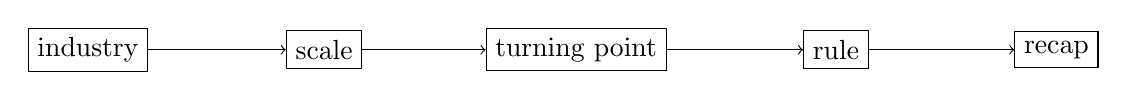
\begin{tikzpicture}
\node[draw, rectangle] (a) at (0,0) {industry};
\node[draw, rectangle] (b) at (3.0,0) {scale};
\node[draw, rectangle] (c) at (6.2,0) {turning point};
\node[draw, rectangle] (d) at (9.5,0) {rule};
\node[draw, rectangle] (e) at (12.3,0) {recap};
\draw[->] (a)--(b);
\draw[->] (b)--(c);
\draw[->] (c)--(d);
\draw[->] (d)--(e);
\end{tikzpicture}
\end{center}
\end{figure}

The lecture will now run that machine several times. Before we follow it case by case, it is worth recording the sample in compact form:

\begin{table}
\begin{center}
\begin{tabular}{lllll}
Case & Industry & Scale & Metric & Mechanism \\
Fashion manufacturer & manufacturing & \(30\)M & best year & rapid COVID pivot \\
Property manager & real estate & \(2.5\)B & managed assets & legal and analytic structure \\
Plastic surgeon & medicine & \(>1\)M & best-year amount & high-ticket differentiation \\
Jewelry manufacturer & manufacturing & \(35\)M & best year & labor spread and automation \\
Software founder & software & \(>4\)M & top-line revenue & concentration and hours
\end{tabular}
\end{center}
\end{table}

We may now follow the lecture in the order in which it teaches us to read these cases.

\section{Speed Under Shock: The COVID Manufacturing Pivot}

The first complete interview is set up biographically before it becomes analytical. We hear of oil and gas, then fashion manufacturing, and only then do we arrive at the crucial number: a best year of \(30\) million dollars. The host immediately asks the right next question, namely what happened that year. The answer is not mystical. COVID arrived, the factory was switched into gowns and masks, and the interviewee says that he became the only factory in Los Angeles making that product at the relevant moment.

A cautious reconstruction of the mechanism is
\begin{equation}
O \propto K\,v\,\sigma,
\end{equation}
where \(O\) is opportunity payoff, \(K\) is preexisting productive capability, \(v\) is pivot speed, and \(\sigma\) is market scarcity.

We should read this equation in the exact spirit of the spoken sequence. The entrepreneur did not create demand from nothing; demand arrived from outside. Nor did he create productive capacity from nothing; capacity was already there. What changed was the mapping between existing capacity and newly scarce goods. The lecture is insisting on speed as the decisive variable.

\subsection{Question \& Answer}

\paragraph{Question.} Why can a small entrepreneur win when a sudden market shock hits?

\paragraph{Answer.} Because the relevant asymmetry is not sheer size but response time. The interviewee says that the small entrepreneur is dynamic and can change quickly, whereas large corporations may take years to catch up. In our notation, a short-lived window is valuable precisely when \(v\) is high before \(\sigma\) has collapsed.

That is already a serious commercial theorem. The large firm may have more capital, but the small firm may own the clock. The host then closes the segment by drawing out that principle: the opportunity was huge not because the world suddenly became generous, but because a temporary shortage met a reconfigurable operator who moved first.

\paragraph{Recap.} The first lesson of the lecture is therefore not ``be adaptable'' in the abstract. It is sharper: when a shock reorganizes demand, a flexible plant combined with rapid execution can turn a short-lived scarcity into a best year.

\section{Control After the Windfall}

The lecture does not leave the first interview at the level of one fortunate year. It immediately asks for the deeper lesson of a fifty-year entrepreneurial life. This is a crucial turn. We move from the making of money to the keeping of position. The interviewee says that he sold a company too early, was happy to receive money at the time, and later saw that company end up on Nasdaq. The point lands because the lecture has already established his credibility through the earlier story.

A compact reconstruction of the logic is
\begin{equation}
U_{\mathrm{future}} \propto E\,\Gamma,
\end{equation}
where \(U_{\mathrm{future}}\) denotes future founder upside, \(E\) is retained equity, and \(\Gamma\) is retained control.

We should not over-mathematize this. The transcript is offering an operating principle, not a theorem of asset pricing. But the principle is clear enough. If early capital arrives at the cost of too much dilution or too much lost authority, then the entrepreneur may capture immediate relief while forfeiting long-duration upside. Hence the repeated insistence: keep your skin in the company, give shares when necessary, but do not lose control.

What the host does well here is to preserve the order of reasoning. He first secures the audience's attention with the dramatic year; only after that does he shift the scale of thought from a single event to the structure of ownership over decades. The recap therefore has real weight: a business can throw off money and yet still be mishandled if its founder exits too cheaply or too early.

\section{Law, Real Estate, and Diversification Within One Field}

The next interview begins with one of the lecture's best surprises. Asked what advice he would give his younger self, the real-estate operator says, ``go to law school.'' The phrase sounds strange on first hearing, and the lecture is wise enough not to resolve it too quickly. Only after we sit with the answer do we hear the explanation: law trains a style of thought, law enters everything done in the business, and the scale of the present operation is enormous,
\begin{equation}
A_{\mathrm{UM}} \approx 2.5\times 10^9 \,\mathrm{USD}.
\end{equation}

The lecture has now changed gears. The first interview emphasized timing under shock. The real-estate interview emphasizes structure. We are no longer looking at a short window in a disrupted market; we are looking at a long-career business whose durability rests on contracts, analysis, and legal form.

\subsection{Question \& Answer}

\paragraph{Question.} Why does a real-estate veteran answer a business question by saying, ``go to law school''?

\paragraph{Answer.} Because, in this segment, legal training stands for disciplined analytic thought. The claim is not that everyone must literally become a lawyer. The claim is that real estate is inseparable from legal and contractual structure, and that one learns a method of reasoning by taking law seriously.

Only after that surprising answer is explained does the host ask about diversification. The resulting resolution is equally precise. One should indeed get very good at one thing, but diversification need not mean leaving the field. It can happen inside the field:
\begin{equation}
D_{\mathrm{within}} = f(T,S,G),
\end{equation}
where \(T\) is property type, \(S\) is asset size, and \(G\) is geography.

This equation is a compact restatement of the interviewee's examples: commercial versus residential, large residential versus small residential, different cities, different states. The lecture's answer to the focus-diversification tension is therefore subtle. We do not oppose specialization and diversification as if they were incompatible. We diversify \emph{within} a mastered domain.

\paragraph{Recap.} The host later compresses this into a larger rhetorical line about law pressing into business whether we like it or not. We should keep the rhetoric in its place. The real substance is simpler and stronger: scale in real estate rests on an analytic style, and breadth becomes safe only when it is breadth inside competence.

\section{High-Ticket Craft and the Refusal To Be Ordinary}

The plastic-surgery segment broadens the lecture's field of examples without changing its method. We again ask industry, scale, and mechanism. This time the business is a high-ticket craft in a crowded prestige market. The interviewee reports a best year north of seven figures,
\begin{equation}
Y_{\mathrm{plastic},\max} > 10^6 \,\mathrm{USD},
\end{equation}
though the transcript does not refine the figure further. He also says that he reached that level very early and that his real decision was not merely to enter the field, but to refuse to be another ordinary person in it.

That distinction matters. In the earlier interviews, the mechanism lay in speed, then in ownership, then in legal structure. Here it lies in position. Los Angeles and Beverly Hills already contain many plastic surgeons. The route to scale is therefore not generic presence. It is to occupy the field at a level of conspicuous seriousness.

The host then notices the Lamborghini, and again the lecture makes a useful move. The car is demoted from premise to consequence. The interviewee's answer is effectively that the luxury object is only a reflection of work. One lives the craft, thinks about it, and lets the visible symbols remain derivative.

\paragraph{Recap.} We may state the principle cleanly. In a high-ticket domain, the premium does not attach automatically to participation. It attaches to differentiation that is deep enough to be believed.

\section{Manufacturing Margin Arithmetic and Operational Leverage}

We now arrive at the most explicitly quantitative interview in the lecture. The jewelry manufacturer says he became a millionaire around age \(35\), stayed in business for \(35\) years, and had a best year of \(35\) million dollars. Asked what took the business from seven to eight figures, he gives a two-part answer: stay current on manufacturing techniques, and understand that the business sells labor rather than commodities.

We begin with the standard bookkeeping identity
\begin{align}
\Pi &= R - C,\\
C &= C_{\mathrm{materials}} + C_{\mathrm{labor}} + C_{\mathrm{overhead}}.
\end{align}

Now let us follow the transcript carefully. The interviewee says that customers know the price of diamonds. They also know the price of gold because it is on the market every day. That means the material side of the sale is largely transparent. The hidden room, if there is any, lies somewhere else.

A cautious reconstruction is therefore
\begin{align}
R &= R_{\mathrm{materials}} + R_{\mathrm{labor}},\\
R_{\mathrm{materials}} &\approx C_{\mathrm{materials}},\\
\Pi_{\mathrm{jewelry}} &\approx R_{\mathrm{labor}} - C_{\mathrm{labor}} - C_{\mathrm{overhead}}.
\end{align}

If overhead is relatively stable across comparable pieces, the lecture pushes us one step further:
\begin{equation}
\Pi_{\mathrm{jewelry}} \approx P_{\mathrm{labor,customer}} - C_{\mathrm{labor,internal}}.
\end{equation}

\begin{proposition}
Under transparent commodity pricing, operational leverage in this business comes mainly from reducing internal labor cost rather than from extracting hidden markups on diamonds or gold.
\end{proposition}

\begin{proof}
\begin{enumerate}
\item Customers know the market prices of the main material inputs.
\item Those inputs therefore behave approximately like pass-through quantities.
\item The interviewee states that the business ``sold labor.''
\item Mechanization and automation primarily act on process efficiency, hence on internal labor cost.
\item Therefore the move from seven to eight figures is most naturally explained by widening the labor spread.
\end{enumerate}
\end{proof}

That is why the next equation has real force:
\begin{equation}
\Delta \Pi_{\mathrm{jewelry}} > 0
\qquad \text{when} \qquad
\Delta C_{\mathrm{labor,internal}} < 0
\end{equation}
provided that customer-facing labor pricing does not fall by the same amount.

\paragraph{Worked example.} Suppose, purely illustratively, that the accepted labor charge on a unit is \(100\) dollars. If internal labor cost falls from \(70\) dollars to \(55\) dollars after mechanization, then the labor spread rises
\begin{equation}
100-70 = 30
\qquad \longrightarrow \qquad
100-55 = 45.
\end{equation}
The margin on labor has increased by \(15\) dollars per unit, or by \(50\%\), without any change in the market quotes of diamonds or gold. The numbers are ours, not the speaker's, but the logic is precisely his.

\subsection{Question \& Answer}

\paragraph{Question.} If customers already see the prices of diamonds and gold, where does the manufacturer actually make money?

\paragraph{Answer.} In labor, more exactly in the spread between the labor price the customer accepts and the internal labor cost the manufacturer must bear. That is why staying current on technique matters, and that is why mechanization matters: both act on the cost side of the only large adjustable spread that remains.

The advice that follows in the interview remains close to this same structure. ``Pay yourself first'' is phrased somewhat roughly in the transcript, but the intended logic is clear enough. Reinvest in the field you know. Bet on yourself in the domain whose economics you understand. Preserve integrity, because once trust is lost even a good cost structure cannot save the business.

\section{Youth, Concentration, and the Long-Hours Doctrine}

The final interview gives the chapter its generational contrast. The founder is \(22\), says he began building companies in middle school, runs a team of about \(30\) people, and expects the current year to exceed four million dollars in top-line revenue:
\begin{equation}
R_{\mathrm{software},\mathrm{top}} > 4\times 10^6 \,\mathrm{USD}.
\end{equation}

The host again uses the same ladder of questions, but the answer now differs in tone from the older operators. The founder's doctrine is concentration. When one is young, he says, one should put one's eggs in one basket and drive that basket hard rather than diffusing attention too early into retirement-style diversification. Long hours are not an ornament on this doctrine; they are part of its mechanism. He says he looks for the same thing in partners and employees.

We should preserve the phase-specific nature of the claim. This is not presented as a timeless law for every balance sheet and every age. It is a rule for a certain stage of life and company-building. The lecture ends, then, not with a universal formula, but with an explicit contrast. The older speakers teach control, staying within competence, and compounding what one already understands. The younger speaker teaches concentration, intensity, and execution speed at the beginning of the curve.

\paragraph{Recap.} That ending is structurally elegant. The lecture began with visible wealth and curiosity. It ends with behavior under time pressure: one basket, many hours, high expectation of oneself and of collaborators.

\section{Summary}

If we read the lecture in the order it teaches itself, a coherent commercial mathematics emerges. We begin with a montage of outcomes, but the host quickly forces us beneath appearances. The first manufacturer teaches us speed under shock:
\[
\text{opportunity} \propto \text{capability}\times \text{speed}\times \text{scarcity}.
\]
The same segment then deepens into a lesson about retained upside:
\[
\text{future upside} \propto \text{equity retained}\times \text{control retained}.
\]
The real-estate operator turns us toward legal structure and diversification within one field. The plastic surgeon shows that premium income may come from refusing to be ordinary in a crowded high-ticket market. The jewelry manufacturer gives the lecture's cleanest derivation, namely that transparent commodity inputs push margin toward labor spread and process efficiency. The young software founder closes the chapter with a doctrine of concentration and hours.

What makes the lecture serious is that it does not let any case remain a mere anecdote. Again and again the host asks for the hidden mechanism and then recaps it as a rule. That is the proper way to read the chapter. We are not being shown cars and neighborhoods for their own sake. We are being shown several different ways in which wealth can arise from timing, structure, differentiation, cost discipline, and effort.